
\section*{Question 4}
\begin{enumerate}[(a)]
    \item We predict the out-of-sample returns based on three different models:
    \begin{enumerate}[i.]
        \item Using dividend-price ratio:
            \begin{equation*}
                    \hat{R}_{t,DP}^e = \hat{\alpha} + \hat{\beta}_{t-1} dp_{t-1}  
            \end{equation*}
        \item Using all the variables from Dong et al. (2022):
            \begin{equation*}
                \hat{R}_{t,OLS}^e = \hat{\alpha} + \sum_{i=1}^{K}\hat{\beta}_{i,t-1} X_{i,t-1}
            \end{equation*}
        \item Using combination-mean forecast:
            \begin{equation*}
                \hat{R}_{t,CM}^e = \frac{1}{K}\sum_{i=1}^{K} \hat{R}_{t,i}^e
            \end{equation*}
            where, for each $i$,
            \begin{equation*}
                \hat{R}_{t,i}^e = \hat{\alpha}_i + \hat{\beta}_{i,t-1} dp_{t-1}
            \end{equation*}
    \end{enumerate}
    where $\hat{\alpha}$ and $\hat{\beta}$ are estimated using OLS regression for the in-sample data which is an expanding window from 1970/01 until the previous month of the out-of-sample period. The out-of-sample period is from 1985/01 until 2017/12. We compare each model using the out-of-sample $R^2$ which is defined as:
    \begin{equation*}
        R^2_{oc} = 1 - \frac{\sum_{t=1}^{T} (R_{t}^e - \hat{R}_{t}^e)^2}{\sum_{t=1}^{T} (R_{t}^e - \bar{R}_{t}^e)^2}
    \end{equation*}
    where $R_{t}^e$ is the realized excess return and $\hat{R}_{t}^e$ is the predicted excess return. The out-of-sample $R^2$ for each model :
    \begin{table}[H]
        \centering
        \begin{tabular}{c|c}
            Model & $R^2_{oc}$ \\
            \hline
            DP & -0.0237 \\
            OLS & -0.6856 \\
            CM & 0.0128 \\
        \end{tabular}
        \caption{Out-of-sample $R^2$ for each model}
        \label{tab:my_label}
    \end{table}
    As we can see, the out-of-sample $R^2$ for the DP and OLS model is negative which means that the DP model is not able to predict better than the benchmark which is the historical mean and the OLS model is worse than the DP model. However, the CM model has a positive out-of-sample $R^2$ which means that it is able to predict better than the benchmark. 

    \begin{lstlisting}[language=Python, caption=Python code for prediction, label={lst:q1a}, escapechar=|, frame=single, basicstyle=\small, showstringspaces=false, captionpos=b, breaklines=true, showspaces=false, showtabs=false, keywordstyle=\color{blue}, commentstyle=\color{gray}]
        data = pd.read_excel("Assignment1Data_G1.xlsx", sheet_name="Predictability")
        data = data.dropna()
        years = range(1970,2018)
        periods = [int(str(i) + "0" + str(j)) for i in years for j in range(1,10) if len(str(j)) == 1]
        periods.extend([int(str(i) + str(j)) for i in years for j in range(10,13) if len(str(j)) == 2 ])
        periods.sort()
        # %% Estimation
        def prediction(X,y):
            beta = sm.OLS(y,X).fit().params.to_numpy()
            return X.iloc[-1].to_numpy() @ beta
        BM_results = {}
        DP_results = {}
        OLS_results = {}
        CM_results = {}
        for prediction_period in tqdm([j for j in periods if j >= 198501]):
            in_sample_period = [i for i in periods if i < prediction_period]
            in_sample_data = data[data["Month"].isin(in_sample_period)]
            X = sm.add_constant(in_sample_data["dp"])
            y = in_sample_data["ExcessRet"]
            BM_results[prediction_period] = y.mean()
            DP_results[prediction_period] = prediction(X,y)
            columns = list(data)
            columns.remove('Month')
            columns.remove('ExcessRet')
            columns.remove('Rfree')
            columns.remove('dp')
            X = sm.add_constant(in_sample_data[columns])
            OLS_results[prediction_period] = prediction(X,y)
            CM_list= []
            for i in columns:
                X = sm.add_constant(in_sample_data[i])
                CM_list.append(prediction(X,y))
            CM_results[prediction_period] = np.mean(CM_list)
    \end{lstlisting}
    
    \item We need to perform the Diebold-Mariano test to test for the statistical significance of the difference between the out-of-sample $R^2$ of the models. The null hypothesis is that the difference between the out-of-sample $R^2$ is zero. The test statistic is defined as:
    
    \begin{equation*}
        DM = \frac{\bar{d}}{\sqrt{\frac{1}{T}\sum_{t=1}^{T}(d_t -\bar{d}_t)^2}}
    \end{equation*}
    where $d_t = \hat{\varepsilon}_t^2 - \tilde{\varepsilon}_t^2$ and $\bar{d}_t = \frac{1}{T_{os}\sum d_t}$. Also, we use the Clark-West test which has a different definition for the $d_t$:
    \begin{equation*}
        d_t = \hat{\varepsilon}_t^2 - [\tilde{\varepsilon}_t^2 -(\tilde{R}_t - \hat{R}_t)^2]
    \end{equation*}
    The calculated test statistics for each model are:
    \begin{table}[H]
        \centering
        \begin{tabular}{c|c|c}
            Model & $DM$ & $CW$\\
            \hline
            DP &  $-1.418$ & $-0.0606$\\
            OLS &  $-5.3738$ & $1.321$ \\
            CM & $0.5262$ & $2.0521$\\
        \end{tabular}
        \caption{Out-of-sample $R^2$ for each model}
        \label{tab:my_label}
    \end{table}

    The critical values for the Diebold-Mariano test are $-1.96$ and $1.96$ for the two-tailed test. Since the test statistics for the DP and CM models are not statistically significant, we cannot reject the null hypothesis that the difference between the out-of-sample $R^2$ is zero. On the other hand, the test statistic for the OLS model is statistically significant which means that the out-of-sample $R^2$ of the OLS model is statistically predict less than benchmark model due to the negative sign of the test statistic. 

    In addition, we can see that the test statistics for the Clark-West test are different from the Diebold-Mariano test. The critical values for the Clark-West test are the same as before. The test statistic for the DP and OLS model are not statistically significant which means that the null hypothesis cannot be rejected. However, the test statistic for the CM model is positive and statistically significant which means that  the model is statistically predicts better than benchmark model.

    \begin{lstlisting}[language=Python, caption=Python code for Diebold-Mariano test, label={lst:q1a}, escapechar=|, frame=single, basicstyle=\small, showstringspaces=false, captionpos=b, breaklines=true, showspaces=false, showtabs=false, keywordstyle=\color{blue}, commentstyle=\color{gray}]
        def DM_test(y_tilde, y_hat):
    T = len(y_hat)
    d = y_tilde**2 - y_hat**2
    delta_hat = np.mean(d)
    # sigma_hat = np.sqrt(np.sum((d - delta_hat)**2)/(T-1))
    # Newey-West correction with on lag
    sigma_hat = np.sqrt(np.sum((d - delta_hat)**2)/(T-1) + 2*np.sum([d[i]*d[i-1] for i in range(1,T)])/(T-1))

    DM = delta_hat/sigma_hat * np.sqrt(T)
    return DM

    def Clark_West_test(y_tilde, y_hat, R_tilde, R_hat):
    T = len(y_hat)
    d = y_tilde**2 - (y_hat**2 - (R_tilde - R_hat)**2)
    delta_hat = np.mean(d)
    # sigma_hat = np.sqrt(np.sum((d - delta_hat)**2)/(T-1))
    sigma_hat = np.sqrt(np.sum((d - delta_hat)**2)/(T-1) + 2*np.sum([d[i]*d[i-1] for i in range(1,T)])/(T-1))
    CW = delta_hat/sigma_hat * np.sqrt(T)
    return CW
    \end{lstlisting}

    \item Now we want to compare the cumulative returns of the portfolios constructed based on the predicted excess returns of each model. The cumulative returns are calculated as:
    \begin{equation*}
        R_{t+1} = R_{t} + \hat{\omega}_{t,j}^*R_{t}^e
    \end{equation*}
    where $\hat{\omega}_{t,j}^*$ is the optimal weight of the portfolio at time $t$ and $j$ is the model. The optimal weights are calculated as:
    \begin{equation*}
        \hat{\omega}_{t,j}^* = \begin{cases}
            2 & \text{if } \hat{\omega}_{t,j} \geq 2\\
            \hat{\omega}_{t,j} & \text{if } -1 < \hat{\omega}_{t,j} < 2\\
            -2 & \text{if } \hat{\omega}_{t,j} \leq -1\\
        \end{cases} \quad \text{where } \quad \hat{\omega}_{t,j} = \frac{1}{\gamma}\dfrac{\hat{R}^e_{t,j}}{\hat{\sigma}^2_{R^e,t}}
    \end{equation*}
    where $\gamma$ is the risk aversion parameter and $\hat{\sigma}^2_{R^e,t}$ is the variance of the predicted excess returns over the last 60 months. The cumulative returns of the portfolios are shown in Figure \ref{fig:my_label}. We can see that the cumulative returns of the portfolios based on the DP and OLS models could not beat the benchmark which is the historical mean. However, the cumulative returns of the portfolio based on the CM model is able to beat the benchmark.

    It is interesting to see that the prediction models during the dot com bubble cannot beat the benchmark. In addition, the DP model lose its power to predict after the dot com bubble which also become worse than OLS model.

    \begin{figure}[htbp!]
        \centering
        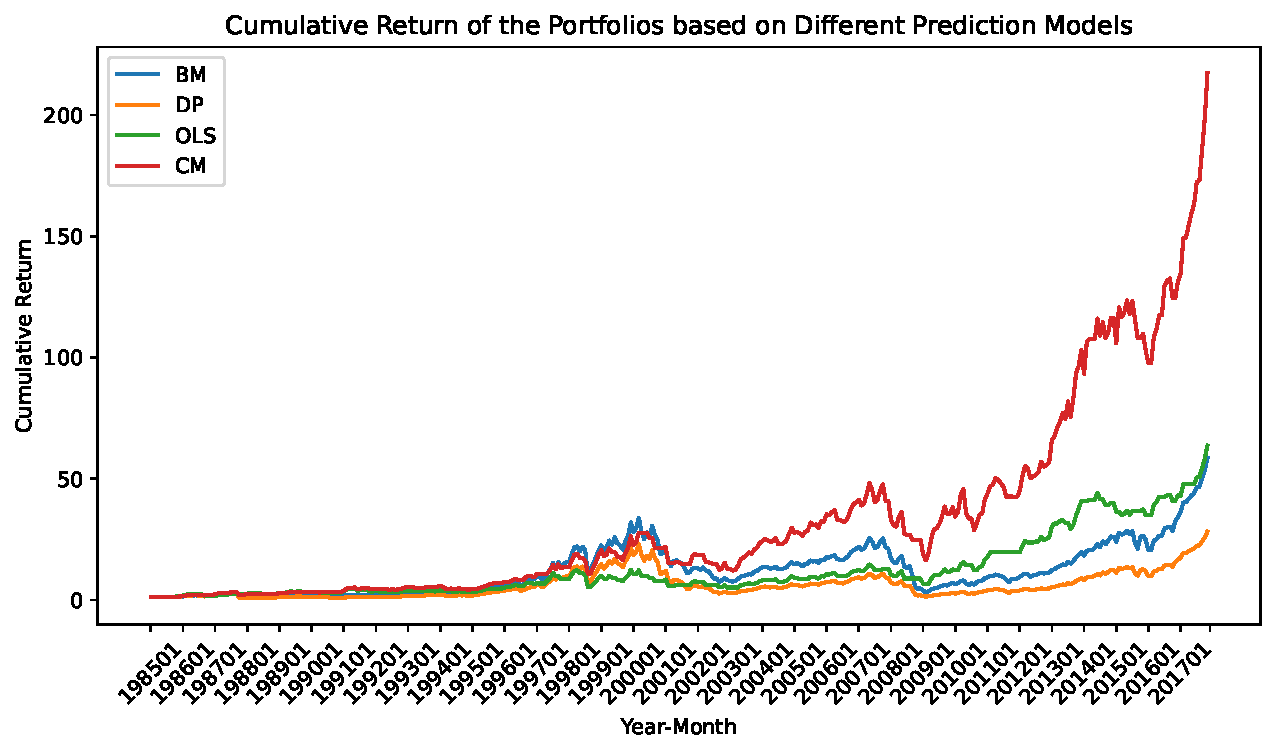
\includegraphics[width=0.85\textwidth]{Out/Ex4_C.pdf}
        \caption{Cumulative returns of the portfolios}
    \end{figure}

    \begin{lstlisting}[language=Python, caption=Python code for portfolio weights, label={lst:q1a}, escapechar=|, frame=single, basicstyle=\small, showstringspaces=false, captionpos=b, breaklines=true, showspaces=false, showtabs=false, keywordstyle=\color{blue}, commentstyle=\color{gray}]
    prediction_data['rolling_var'] = prediction_data.ExcessRet.rolling(60).var()
    gamma = 2
    for prediction_model in ['BM',"DP", "OLS", "CM"]:
        prediction_data['omega_hat'] = prediction_data[prediction_model]/prediction_data['rolling_var']/gamma
        prediction_data['omega_hat_'+prediction_model] = prediction_data['omega_hat']
        prediction_data.loc[prediction_data.omega_hat >= 2,'omega_hat_'+prediction_model] = 2
        prediction_data.loc[prediction_data.omega_hat <= -1,'omega_hat_'+prediction_model] = -1
        prediction_data['r_p_'+prediction_model] = prediction_data['ExcessRet'] + prediction_data['omega_hat_'+prediction_model]*prediction_data['ExcessRet']
    \end{lstlisting}

    \item Now we want to plot the optimal weights of the portfolios. The optimal weights are calculated as mentioned before. The optimal weights of the portfolios are shown in following Figure. We can see that the optimal weights of the portfolios based on the OLS and CM models are not stable and they change over time. However, the optimal weights of the portfolio based on the BM and DP  are stable and they do not change over time. It is interesting to see that the weights from the DP model and the BM model are highly correlated. 
    \begin{figure}[htbp!]
        \centering
        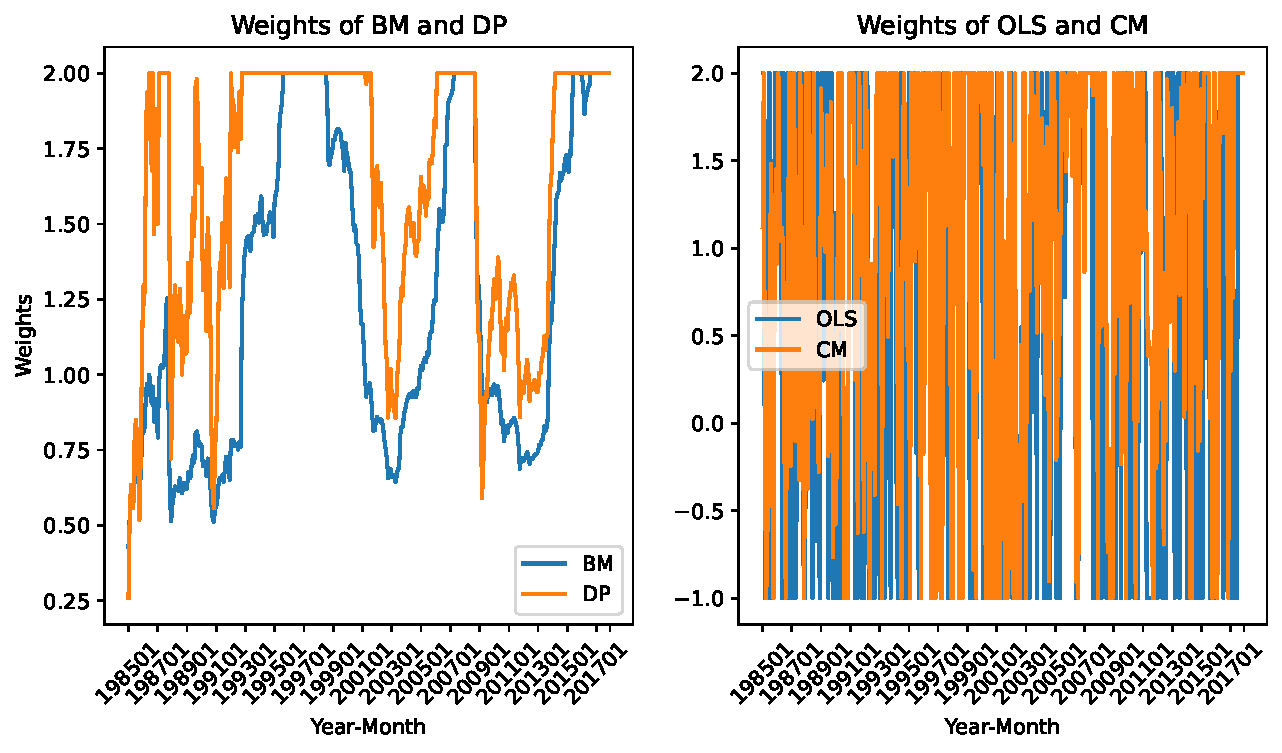
\includegraphics[width=0.85\textwidth]{Out/Ex4_D.pdf}
        \caption{Optimal weights of the portfolios}
    \end{figure}

    \item Now we define a utility function for the investor as:
    \begin{equation*}
        U(\hat{R}_{p,t}^j) = \hat{E}\left[\hat{R}_{p,t}^j\right] - \frac{\gamma}{2} \hat{Var}\left(\hat{R}_{p,t}^j\right)
    \end{equation*}
    and we want to compare the utility of the portfolios based on the predicted excess returns of each model with the utility of the benchmark which is the historical mean. The utility gain is defined as:
    \begin{equation*}
        UG = U(\hat{R}_{p,t}^j) - U(\hat{R}_{p,t}^{BM})
    \end{equation*}
    
    The utility gain for each model is shown in the following table. We can see that the utility gain for the DP model is negative which means that the utility of the portfolio based on the DP model is less than the utility of the benchmark. However, the utility gain for the OLS and CM models are positive which means that the utility of the portfolios based on these models are higher than the utility of the benchmark.

    In this comparison,  we can see that the utility gain for the CM model is the highest which means that the portfolio based on the CM model is the best portfolio among the other portfolios.

    \begin{table}[htbp]
        \centering
        \begin{tabular}{c|c}
            Model & $UG$ \\
            \hline
            DP & -0.003 \\
            OLS & 0.0013 \\
            CM & 0.0043 \\
        \end{tabular}
        \caption{Utility gain for each model}
    \end{table}


\end{enumerate}